\chapter{統計モデル}
この章ではついにデータが登場する。データは母集団から無作為抽出によって得られた数値であるとする。
データを大文字の$X_1,X_2,\cdots,X_n$とし、モデルからサンプリングした確率変数を小文字の$x_1,x_2,\cdots,x_n$とする。
統計モデルはデータの出現頻度や統計量などを予測する。
まず、その予測可能なことについて列挙する。モデルとデータが異なる場合つまり、データの出現頻度をデータが予測できない場合に生じることについて説明する。

\section{正規分布を含んだ統計モデル}
次の3つを仮定したモデルを正規モデルと呼ぶ。
\begin{quote}
    \begin{enumerate}[(1)]
    \item 独立同分布
    \item その分布は、正規分布
    \item 正規分布の母数(平均と分散)はそれぞれ$\mu,\sigma^2$。
    \end{enumerate}
\end{quote}
この正規モデルを$M(\mu,\sigma^2)$と書く。$\sigma^2$をある特定の値にしたときのモデルを$M(\mu)$とし、$\mu$を特定の値にしたモデルを$M(\sigma^2)$とする。

%\subsection{最尤推定量を使ったモデル}
母集団から無作為抽出した標本を元にモデルを構築する。具体的には、$\mu_{ML}=\bar{X},\sigma^2_{ML}=\frac{1}{n}\sum(X_i-\bar{X})$とし、統計モデル$M(\mu_{ML},\sigma^2_{ML})$を最尤モデルと呼ぶ。

以下では、$M(\mu)$による予測について説明する。

\if 0 
このモデルにおいて、統計量$Z(\bar{x},\mu)$の$95\%$予測区間を求める。
%よく入る区間の式を変形し、データを得たときに、そのデータを基準にした$\mu$の範囲に変形してみます。
\begin{eqnarray*}
 & -z_{0.025} < Z(\bar{x},\mu)<z_{0.025} \\
\rightarrow & -z_{0.025} < \frac{\sqrt{n}(\bar{x}-\mu)}{\sigma}  <z_{0.025} \\
\rightarrow & \bar{x}- z_{0.025}\frac{\sigma}{\sqrt{n}} < \mu < \bar{x} + z_{0.025}\frac{\sigma}{\sqrt{n}}
\end{eqnarray*}
\fi

\if 0

\section{問題意識}
確率変数$x_1$または、$x_1,x_2,\cdots,x_n$を得たとき、それらが独立同分布に従うという前提のもと、ある母数をもつ分布関数に従う、または従わないと推測することは可能であるだろうか。
最尤推定から、確率変数を得たなら、最尤推定を行って、母数を推測可能な場合がある。
具体的には、正規分布から得られた確率変数については、その平均と分散は、$(\mu,\sigma^2)=(\bar{x},\sum_{i=1}^{n} (x_i-\bar{x})^2/n)$である。

この問題に対して、
正規分布から確率変数を得たとき、ある母数平均$\mu$をもつ正規分布からサンプリングされていないということはできるだろうか。これを議論する。

%\subsection{問題点}
%aa
\fi

\subsection{データが出現しやすい区間}
ある決められた確率でデータが出現するとモデルが予測する区間を予測区間という。
割合として、よく使われる$95\%$を設定したものを$95\%$予測区間という。
正規分布を含んだモデル$M(\mu)$において、予測区間は比較的簡単に求めることができる。
具体的には、正規分布の規格化を行い、標準正規分布に従うように変換を行い、$\frac{x-\mu}{\sigma}$であるので、予測区間は、
\begin{eqnarray*}
    %-z_{0.05} <\frac{x-\mu}{\sigma} <z_{0.05} \\
    \mu-z_{0.05}\sigma < x < \mu+z_{0.05}\sigma
\end{eqnarray*}
である。この範囲に$95\%$のデータが生じることをモデルが予測する。実際にそのようになるかは不明であり、予測であることを意識した方が良い。

$68\%$の確率でデータを含むと予測する区間が求められる。
\begin{eqnarray*}
    %-z_{0.05} <\frac{x-\mu}{\sigma} <z_{0.05} \\
    \mu-\sigma < x < \mu+\sigma
\end{eqnarray*}

\subsubsection{母集団の標本が指数分布的に分布していた場合}
母集団の分布形と統計モデルに含まれている確率分布関数が著しく異なる場合を考える。
母集団分布として、指数分布を仮定しする。これは、自然から指数分布的なデータが得られたときのことを想定している。
これを予測するモデルを正規分布の仮定されたモデルとする。
\if 0
を使い、最尤モデルにおける平均値は、
$\bar{x}\sim N(\mu_{ML},\sigma^2_{ML}/\sqrt{n})$である。
このことから、モデルは、$\left[ \mu_{ML}-z_{0.05}\sigma_{ML},\mu_{ML}+z_{0.05}\sigma_{ML} \right]$
の間に、$68\%$の確率で平均値が入ることを予測する。
\fi
最尤モデルは、$M(\mu_{ML},\sigma^2_{ML})$である。ここから、
\begin{eqnarray*}
    %-z_{0.05} <\frac{x-\mu}{\sigma} <z_{0.05} \\
    \mu_{ML}-\sigma_{ML} < x < \mu_{ML}+\sigma_{ML}
\end{eqnarray*}
が$68\%$予測区間になる。
言い換えれば、標準偏差の間に、サンプルの平均が入る確率が$68\%$であることをモデルが予測している。
このことを数値シミュレーションにより確かめる。
指数分布からランダムサンプリングを行い、無作為抽出によりサンプルサイズ$10^6$の標本を得たとする。
サンプルが上記の区間に入っている割合を計算する。

\begin{lstlisting}
N = 10**6
sample = expon.rvs(scale=10,size=N)
#sample = norm.rvs(loc=0,scale=1,size=N)
lambd= np.average(sample)
print(np.average(sample),np.std(sample),np.var(sample))

mu = np.average(sample)
s = np.std(sample)

a,b = mu-s,mu+s
len(sample[np.where( (sample >a) & (sample<b) )])/N
\end{lstlisting}
この結果、期待していた値$68\%$よりも著しく大きな確率$86\%$程度を得る。
これは、モデルでは、正規分布を仮定していたが、実際には指数分布的なデータだったために生じる予測の間違いである。
以上でわかるのは、統計モデルと実際の母集団が乖離している場合には、標準誤差に間違いが多くなるということである。

\subsubsection{エラーバー(SD)から読み取れること}
正規分布と指数分布それぞれからサンプルサイズ$N=100$の標本を作り、プロットした(図\ref{fig:sample_norm_expon_model})。それぞれの分布の右側のエラーバーは、$68\%$予測区間。
標本が正規分布であるときには、$68\%$予測区間の中におよそ$68\%$のデータが含まれている。
一方で、標本が指数分布であるときは、モデルの予測と乖離する。このことは、図から読み解くことが難しい。

エラーバー(SD)だけが描かれた図を見るとデータに対する印象が変わる(図\ref{fig:model_predict_SD})。
図\ref{fig:model_predict_SD}には、正規分布と指数分布から得られた標本から、最尤推定を行ったモデル$M(\mu_{ML},\sigma^2_{ML})$における$68\%$予測区間を描画している。
データが正規分布的であるならば、データが区間に入っている割合が予測と一致する。
一方で、データが指数分布的であるならば、モデルの予測(エラーバー)から得られることと、実際のデータは乖離する。
エラーバーからは、中央からデータが対称に分布しており、その中に、$68\%$のデータが入っていることを読み取れる。
実際のデータは図\ref{fig:sample_norm_expon_model}にある通りであり、モデルの予想とは一致しない。

エラーバーにSDを描くときには、特に指定がない限り、正規分布を仮定したモデルを想定しているということが予想される。
実際には、モデルを考えてエラーバーを書いていると断言しがたい。
SDが描かれているのに、検定においては正規分布を仮定しない統計モデルを使っていることも多々ある。
データの描画においては、正規分布を仮定しているにもかかわらず、統計においてはその仮定による推測をやめている。
この場合、著者が何を考えてSDを描いたのか判別しにくい。
%また、データが正規分布的であることに確信を得ることは、サンプルサイズを大きくした標本から想像するしかなく、費用がかさむので行われない。
%このこと、モデルの予測が当たることを肯定できる根拠がないことを意味する。

測定の精度の良さを示す指標としてSDを書くことがある。この場合、ただ単にSDが小さければ良い。
%データが正規分布であるという強い前提がある。

\begin{figure}
    \begin{center}
        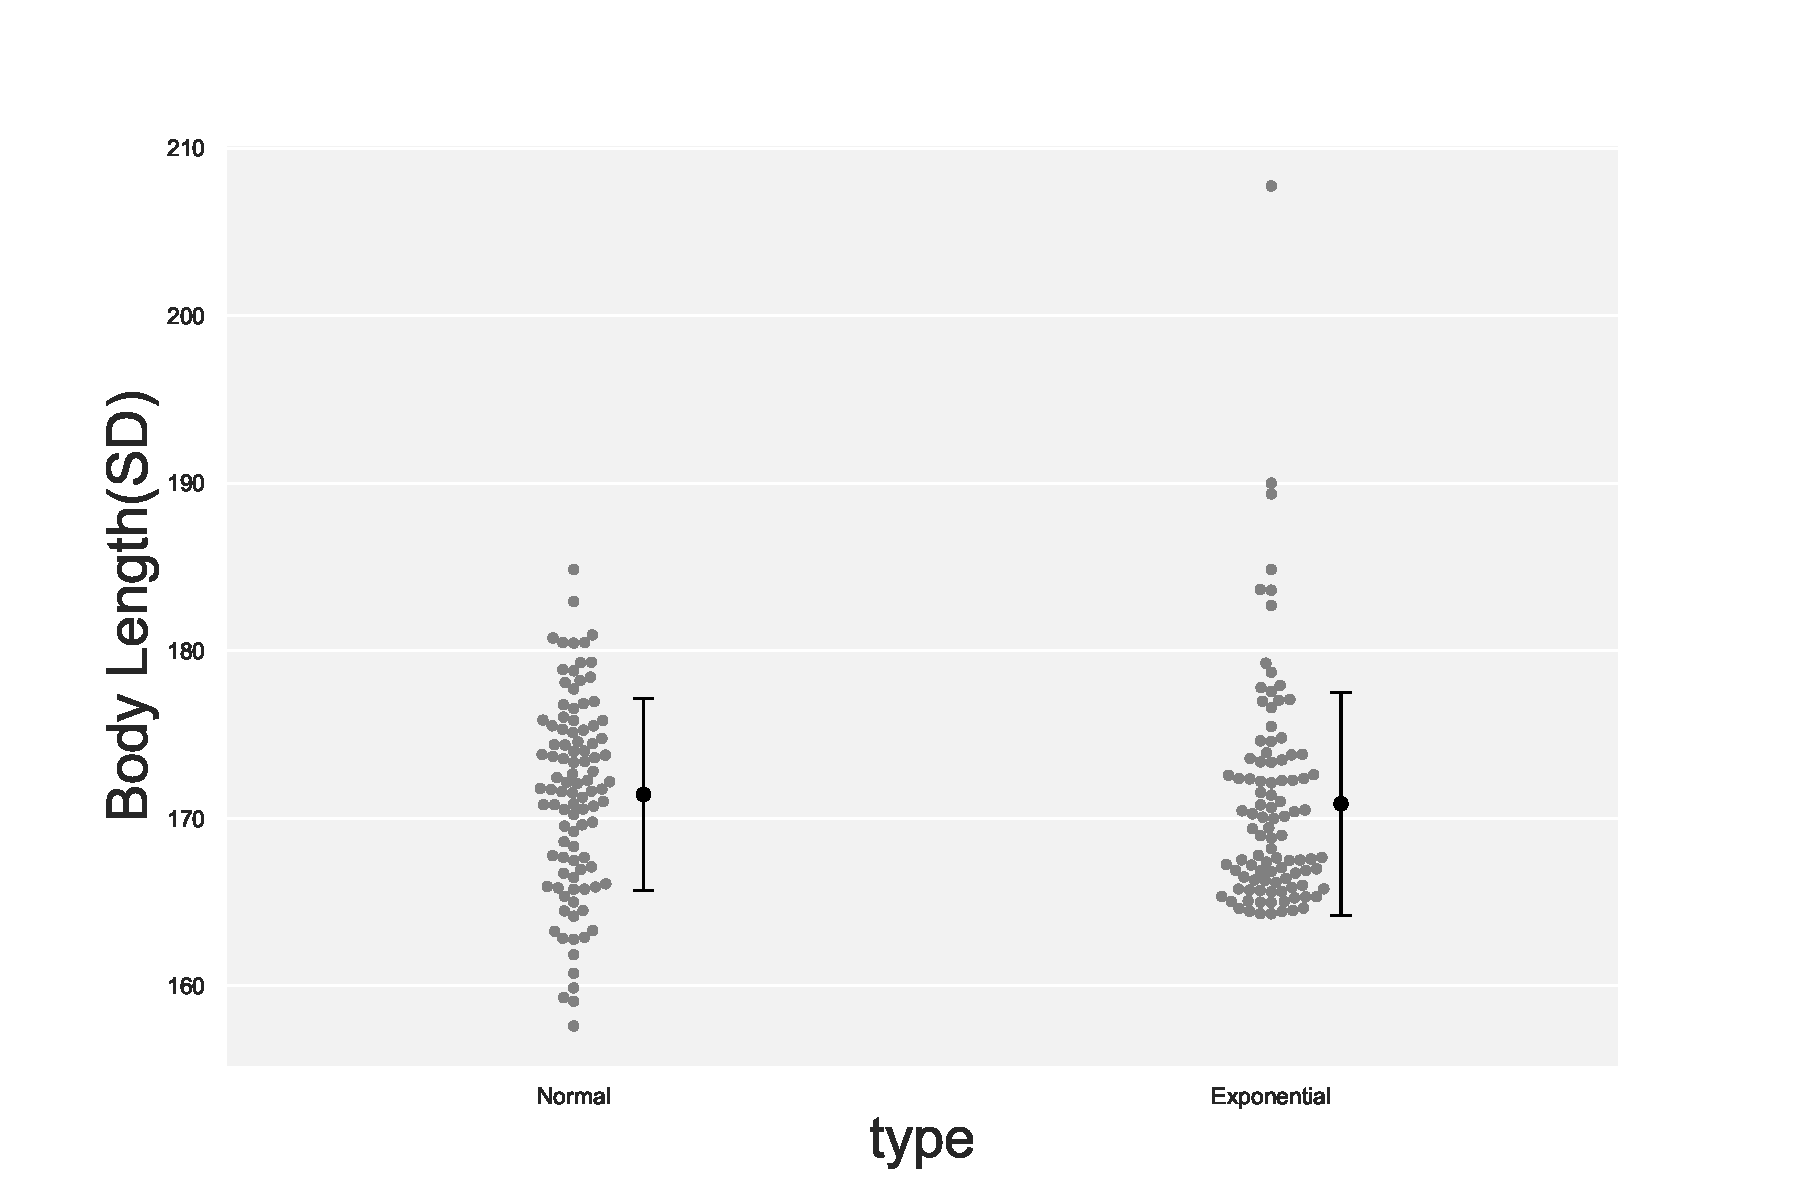
\includegraphics[width=15cm]{./image/12_/sample_norm_expon.pdf}
        \label{fig:sample_norm_expon_model}
        \caption{正規分布と指数分布それぞれからサンプルサイズ$N=100$の標本をプロットした。それぞれの右側にあるエラーバーは、正規分布モデルが予測した$68\%$予測区間。}
      \end{center}
    \end{figure}


\begin{figure}
    \begin{center}
        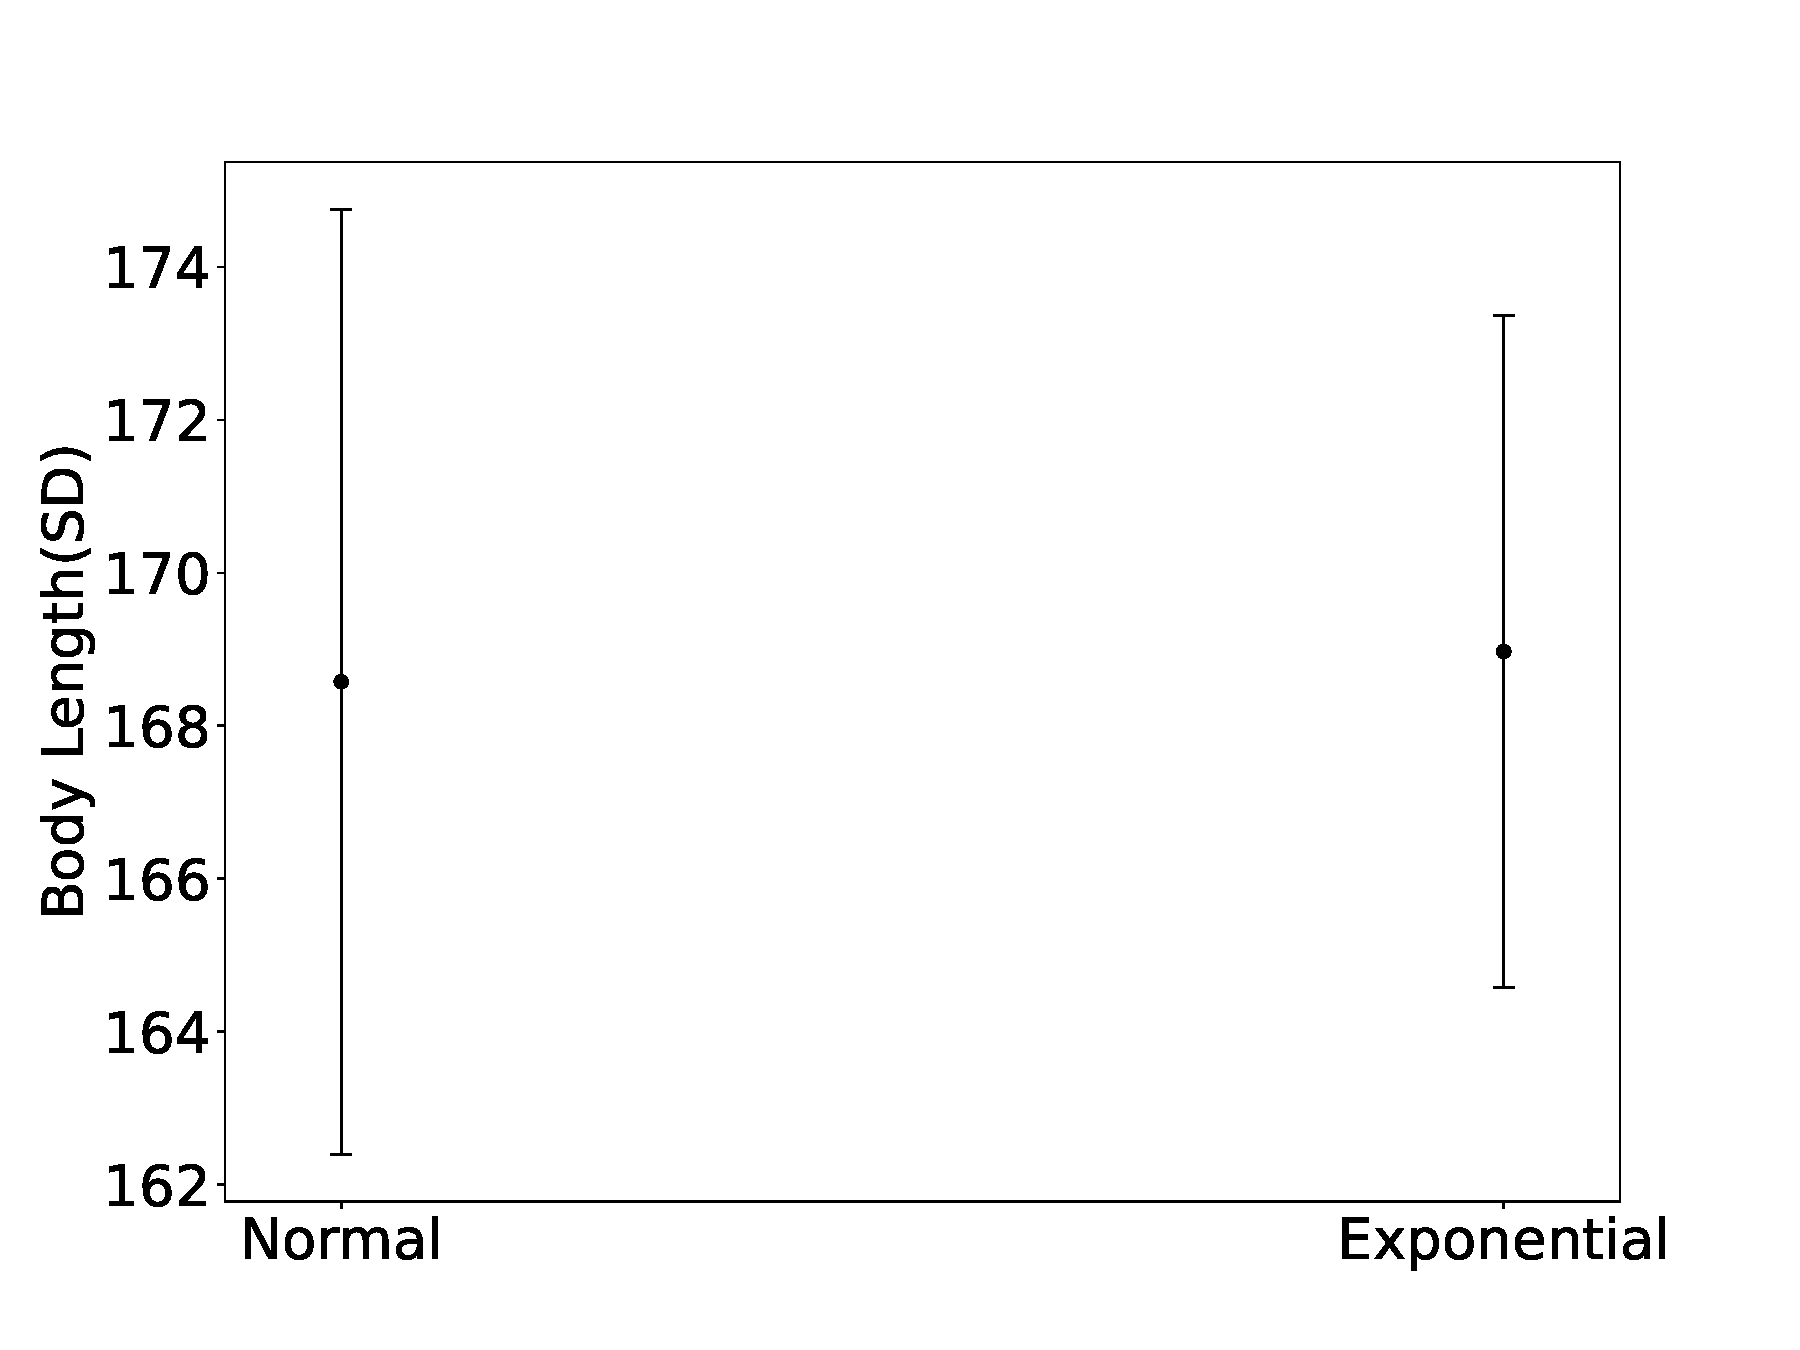
\includegraphics[width=15cm]{./image/12_/model_predict_SD.pdf}
        \label{fig:model_predict_SD}
        \caption{正規分布と指数分布それぞれからサンプルサイズ$N=100$の標本を得た。その標本から推測される$68\%$予測区間を描画した。}
      \end{center}
    \end{figure}


\subsection{平均値が出現する区間}
今回考えている統計モデル$M(\mu)$では、次の統計量$Z$が標準正規分布$N(0,1)$に従うことが、正規分布の再生性によってわかっている。
$$
Z(\bar{x},\mu)=\frac{\sqrt{n}(\bar{x}-\mu)}{\sigma} \sim N(0,1)
$$
ここで$\bar{x}$は、統計モデル$M(\mu)$からサンプリングした標本の標本平均値(データの平均値ではない)、$\mu,\sigma$は統計モデルで設定した母数平均、母数分散。
%$Z(\bar{x},\mu)$が$N(0,1)$に従うということから、$Z(\bar{X},\mu)$が$N(0,1)$における出現頻度が計算できる。
\begin{figure}
    \begin{center}
        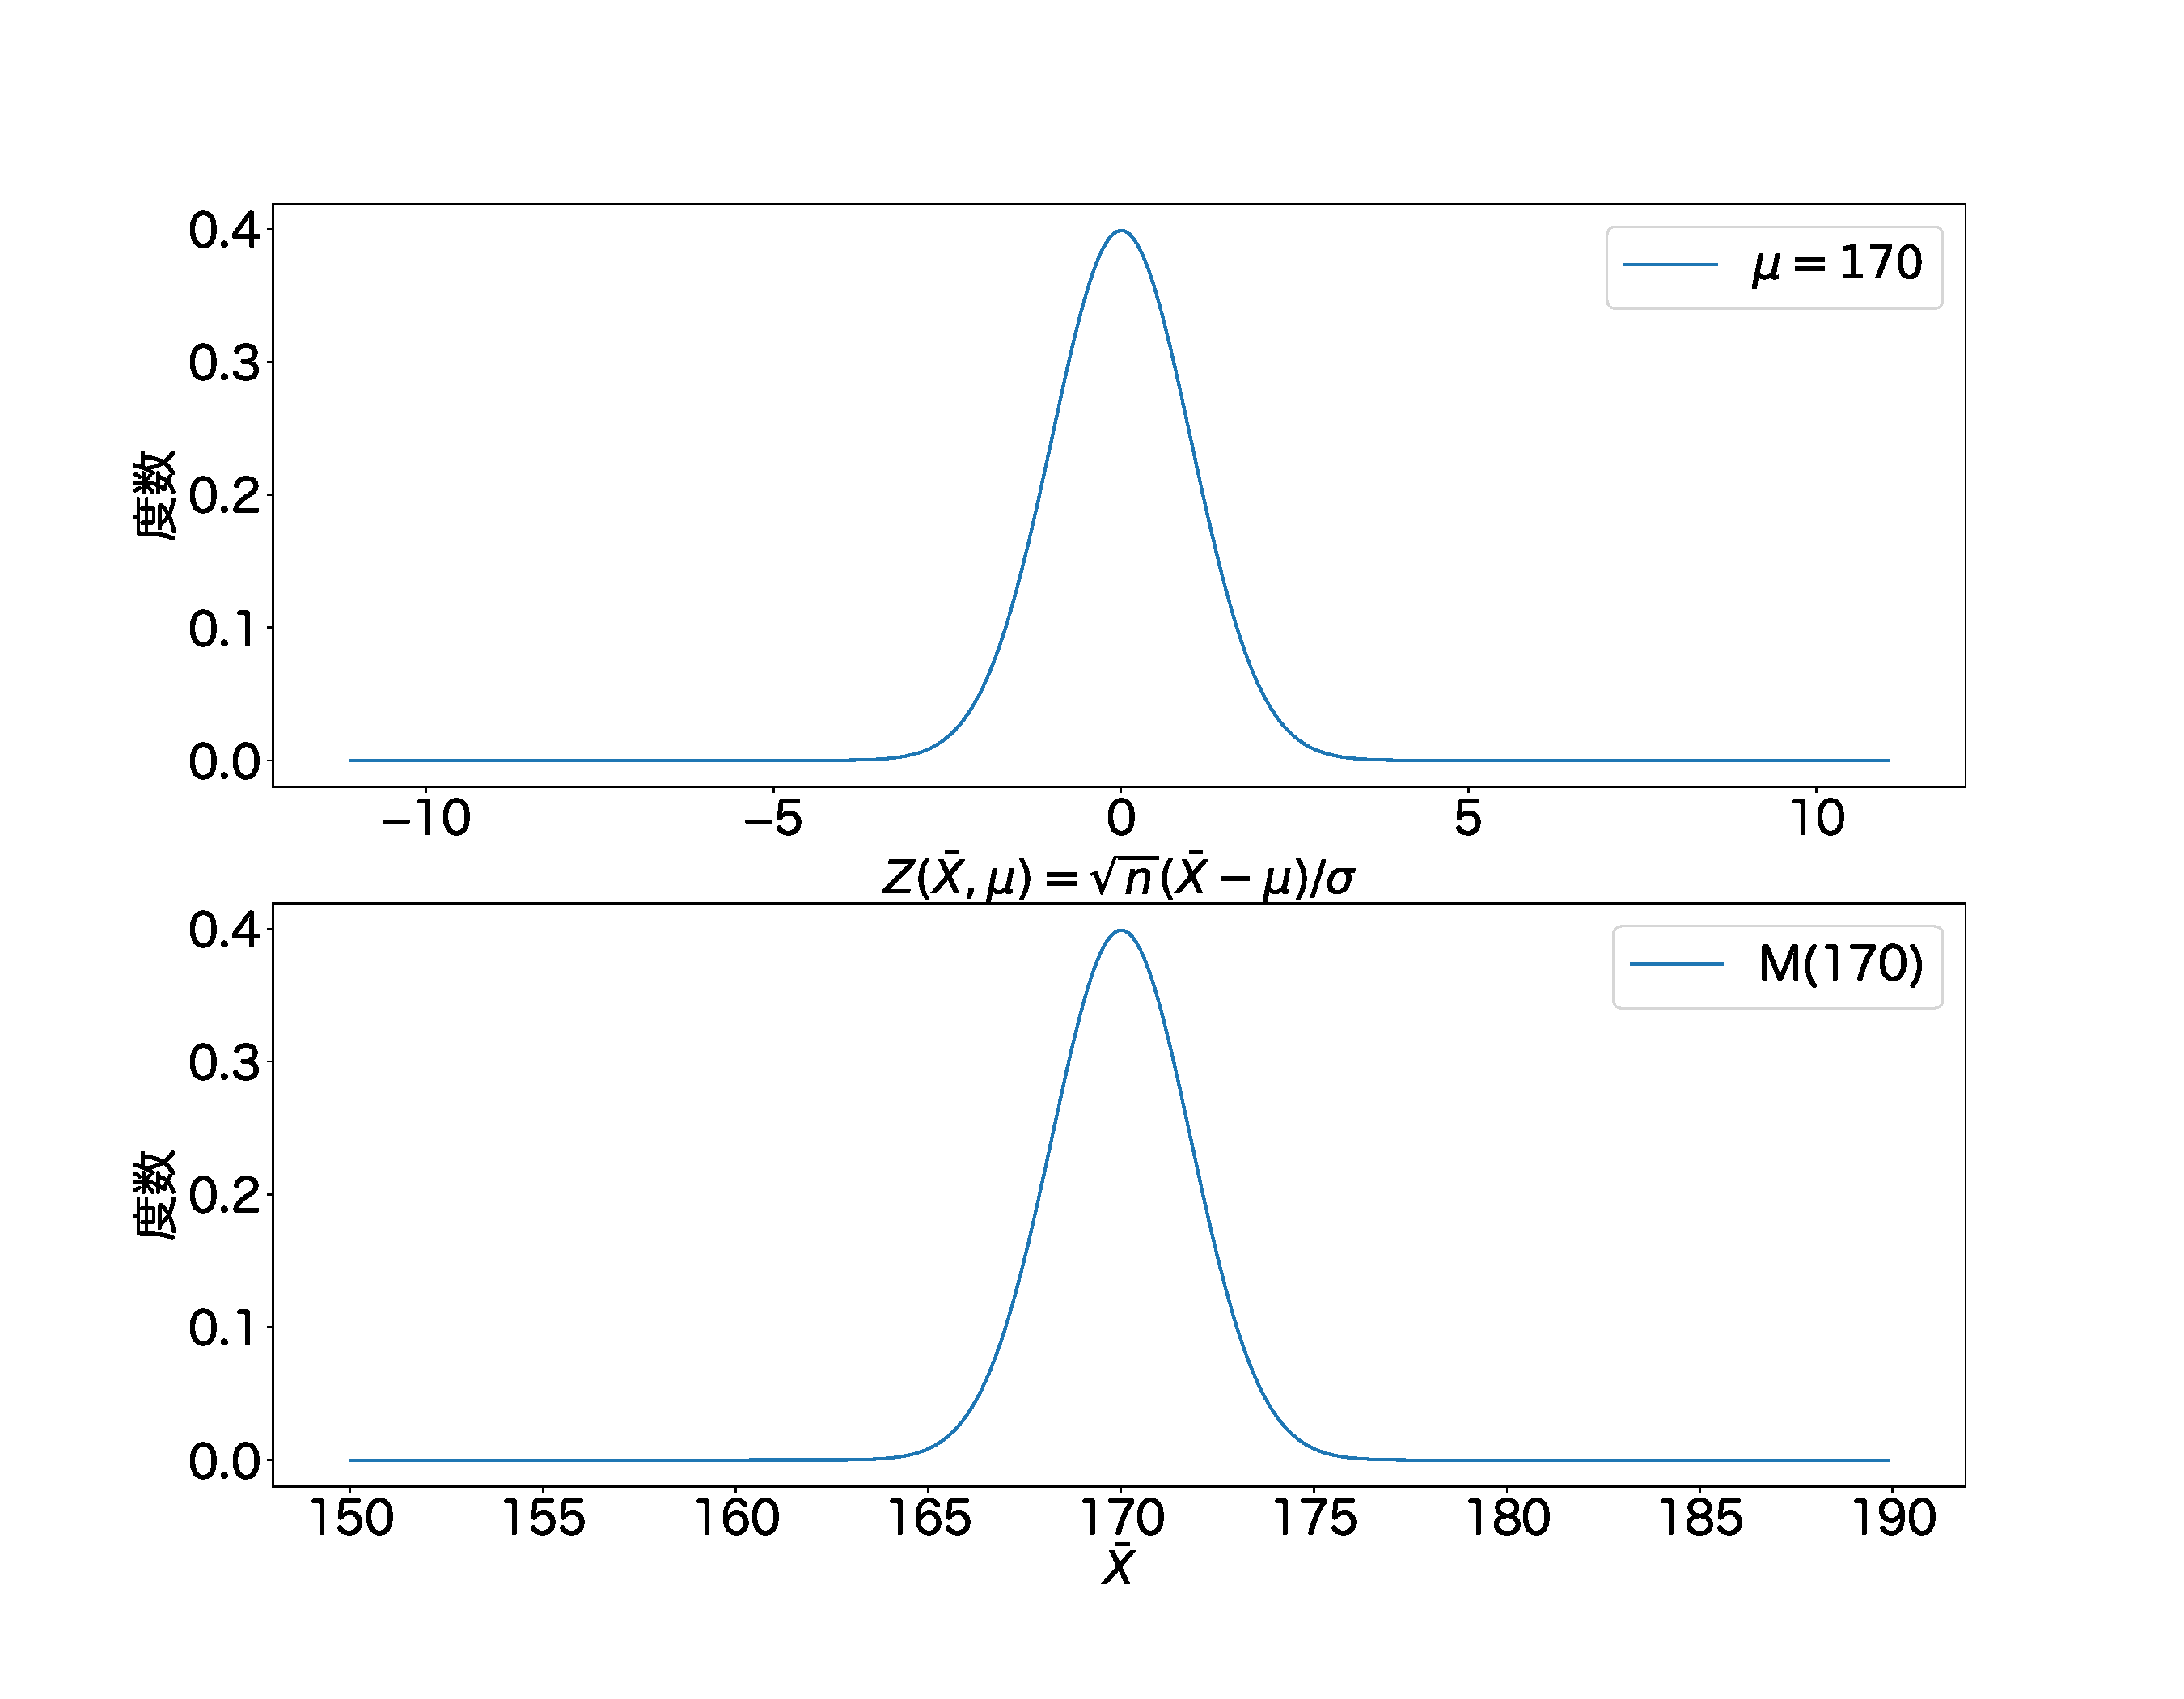
\includegraphics[width=15cm]{./image/03_/normal_Z_frequency.pdf}
        \label{fig:cm_standard_normal_distribution}
      \end{center}
    \end{figure}

$Z$の出現頻度を$Z$または$\bar{x}$の値に応じて書いたものが図\ref{fig:cm_standard_normal_distribution}である。
$Z(\bar{x},\mu)$の$95\%$予測区間が次のように求められる。
$$
-z_{0.025}<Z(\bar{x},\mu)<z_{0.025}
$$
これは、サンプリングされた標本の統計量$Z(\bar{X},\mu)$が$95\%$の確率で得られる範囲である。
統計モデルを使った判断でよく出てくる確率として分野を問わず、$95\%$が使われる。
%この値には身長に関する経験を使わずに決定しています。


$Z(\bar{X},\mu)$を式変形することで、標本平均が$95\%$の確率で出現する区間が推定できる。式を変形する。
\begin{eqnarray*}
    & -z_{0.025} < Z(\bar{X},\mu)<z_{0.025} \\
\rightarrow & -z_{0.025} < \frac{\sqrt{n}(\bar{X}-\mu)}{\sigma}  <z_{0.025} \\
\rightarrow & \mu - z_{0.025} \frac{\sigma}{\sqrt{n}} < \bar{X} < \mu + z_{0.025} \frac{\sigma}{\sqrt{n}}
\end{eqnarray*}
この統計モデルからサンプリングした標本の標本平均$\bar{x}$が$95\%$の確率で見つかる範囲のことを$95\%$信頼区間という。これも、モデルの予測である。

\subsubsection{サンプルサイズによる影響}
$95\%$信頼区間を見てわかるように、サンプルサイズ$n$が大きくなれば、$\bar{x}$が入る範囲は狭くなる。
信頼区間がサンプルサイズに依存することを数値的に確認する。
図\ref{fig:confidence_interval_n}は、信頼区間が$N$に応じて変化する様子を図示した。

\begin{figure}
\begin{center}
    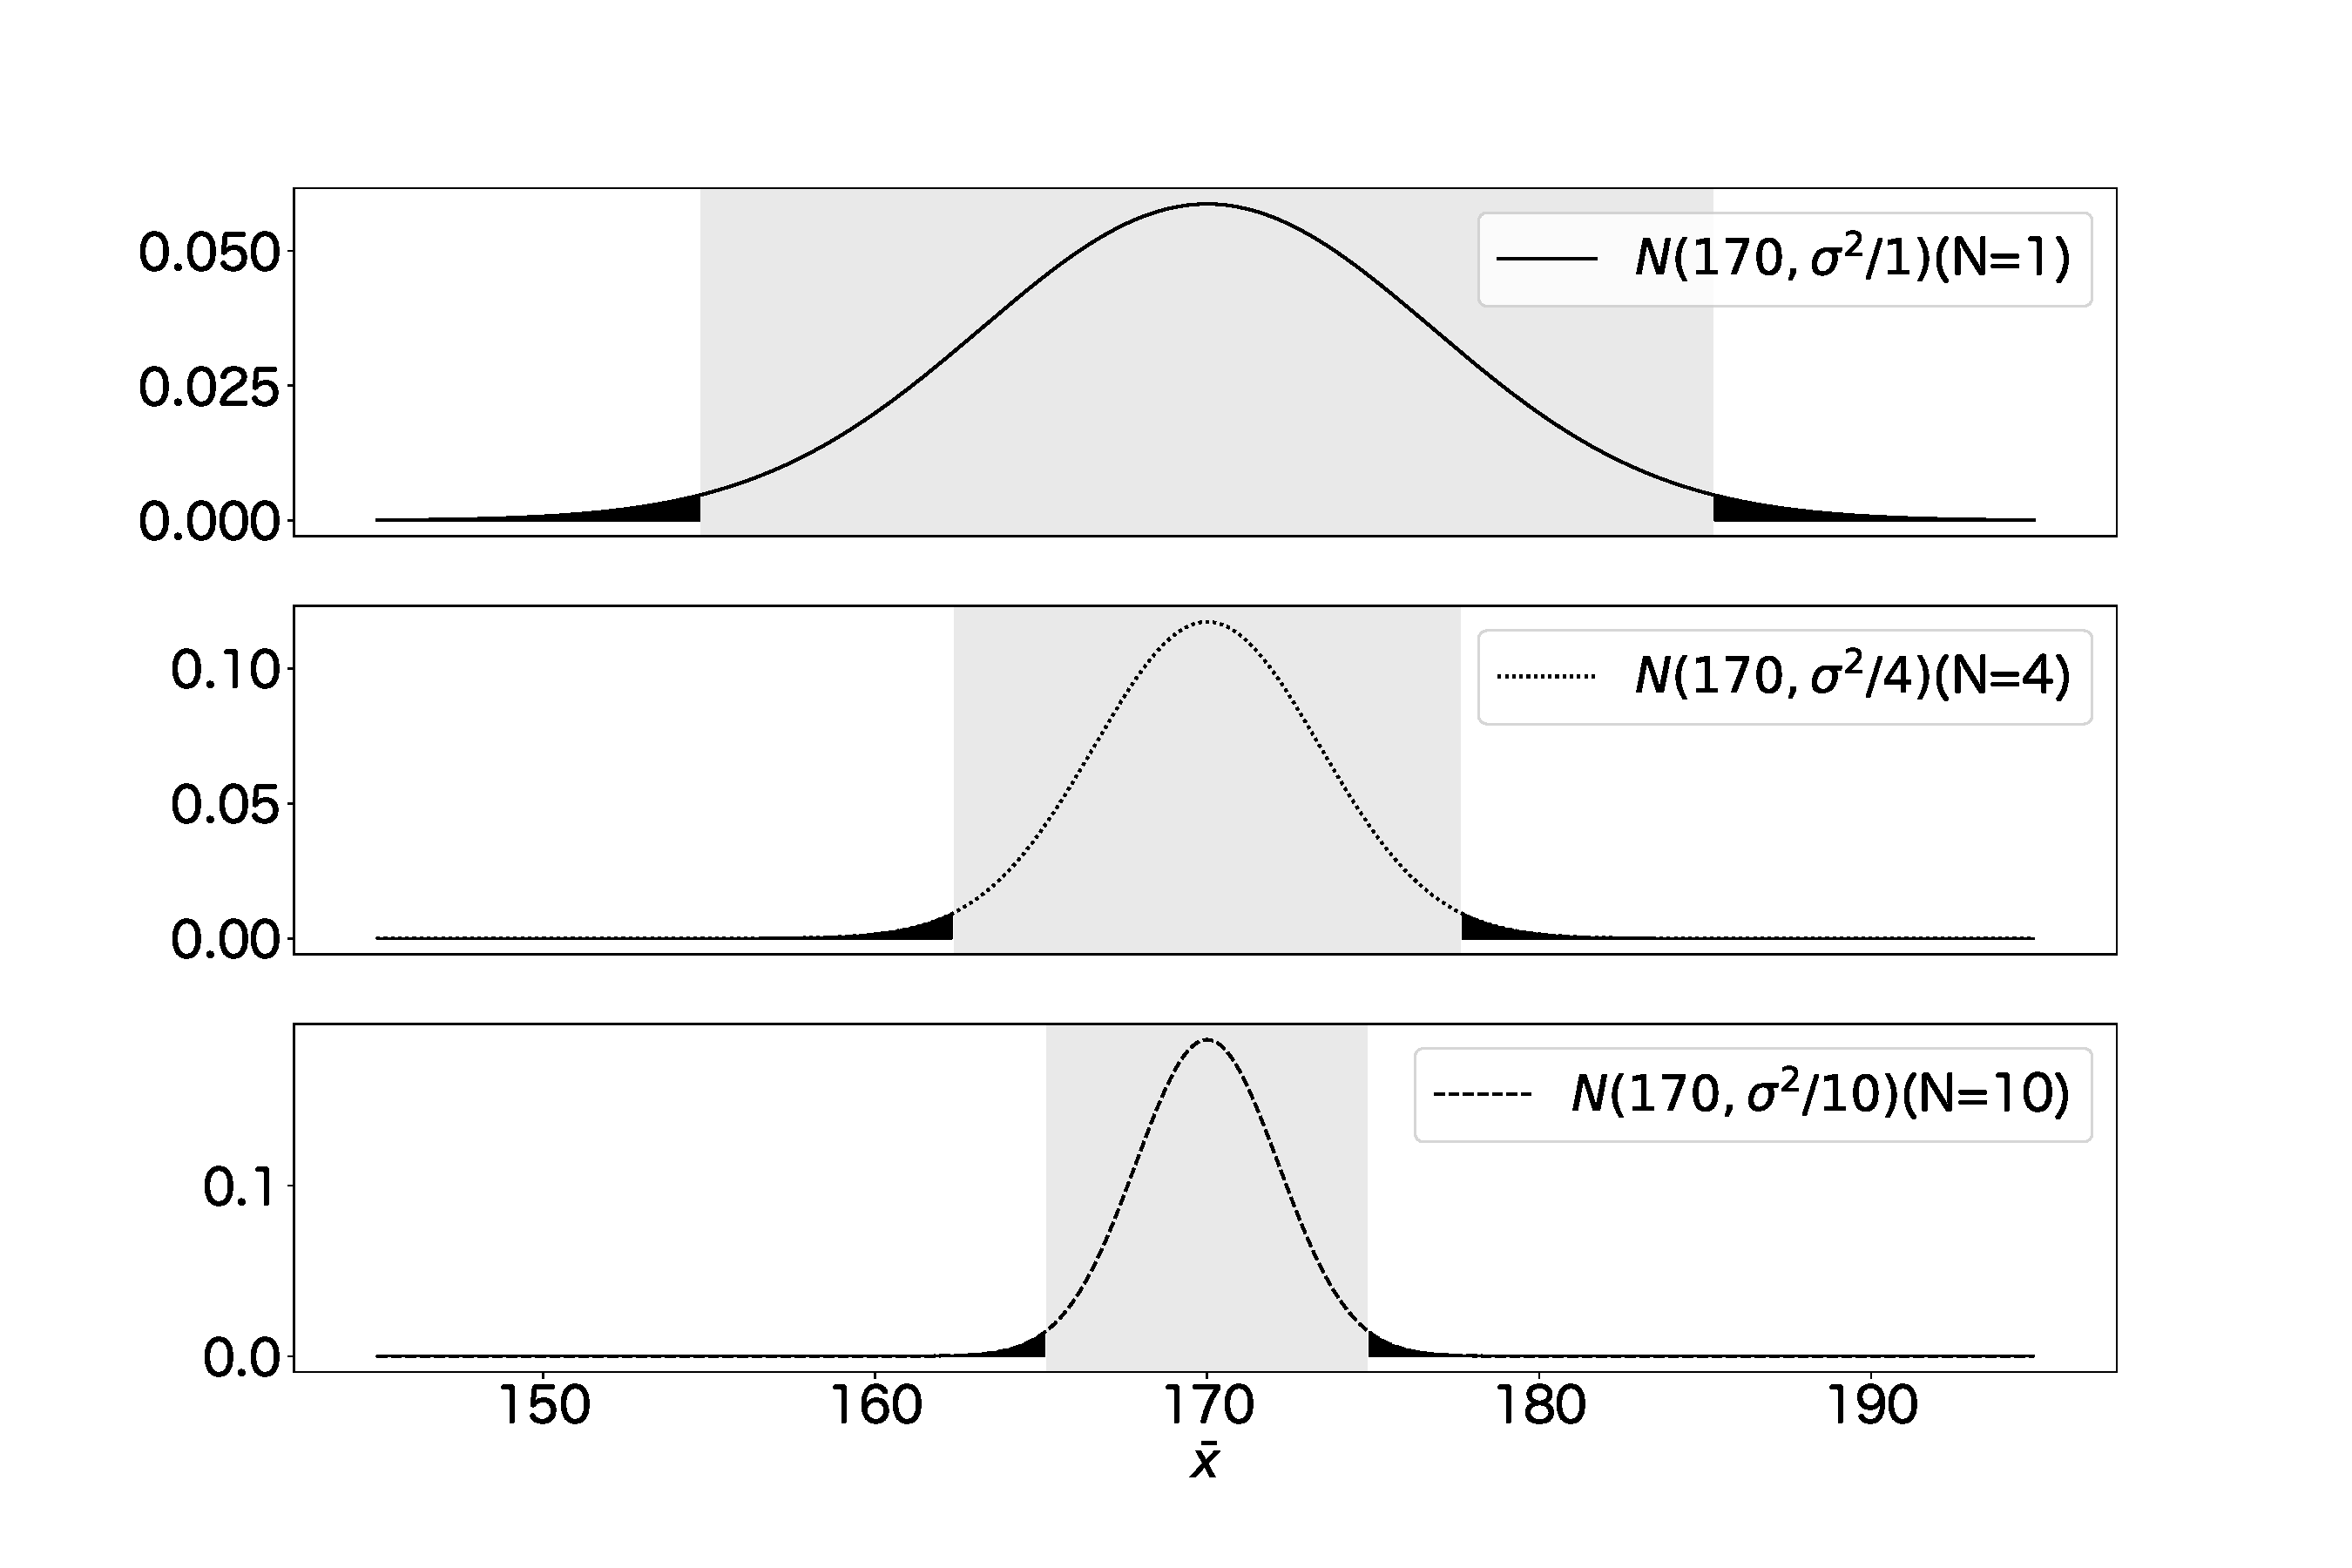
\includegraphics[width=15cm]{./image/03_/confidence_interval.pdf}
%    \caption{信頼区間}
    \caption{(A)$N=1$,(B)$N=4$,(C)$N=10$での信頼区間}
    \label{fig:confidence_interval_n}
  \end{center}
\end{figure}

\if 0
\begin{framed}
    まとめ、
    \begin{itemize}
        \item 統計モデル$M(\mu)$によってサンプリングし、標本を得たとき、標本平均値のよくある値の範囲が信頼区間
    \end{itemize}
    \end{framed}
\fi


\if 0
 川久保統計学P.166
 \fi


%![Z値の頻度]()

信頼区間の中に標本平均が含まれていることは、標本がモデルにり推測可能であることの証拠の一つになる。
ただし、証拠の一つであり、このことは実際には複合的に指標を見て判断する必要がある。
%$\bar{X}$が$95\%$信頼区間の中に入っていることは、この統計モデル
%信頼区間の中に統計量があれば、
%このことから、統計モデル$M(\mu)$でサンプリングしたときに、$95\%$の確率で、この範囲に平均値$\bar{X}$がえられます。


%標本$1$標本$2$について、これを計算してみる。平均値は、それぞれ172.4, 169.0です。
\if 0
標本では、$168.9 < \mu < 176.0$、
この範囲にある$\mu$をもつ統計モデルであれば、この標本によって棄却されない。
%標本$2$では、$165.5 < \mu <172.6$です。
例えば、このモデル$M(\bar{x})$の信頼区間であれば、$M(168)$は棄却できない。
\fi

\if 0
まとめ、
\begin{framed}
    \begin{itemize}
        \item 統計モデル$M(\mu)$のサンプルの平均が$95\%$の確率で入る範囲$\mu - z_{0.025} \frac{\sigma}{\sqrt{n}} < \bar{X} < \mu + z_{0.025} \frac{\sigma}{\sqrt{n}}$。現実の母集団が統計モデルによってよく推測できるなら、この範囲に平均値が入る確率は$95\%$に近くなることもある。逆に、統計モデルが現実をよく捉えることができなければ、母集団から無作為抽出した標本の平均値はこの範囲に入ることは少なくなる。
        \item データがよくある範囲に入る統計モデル$M(\mu)$の$\mu$の範囲$\bar{x}- z_{0.025}\frac{\sigma}{\sqrt{n}} < \mu < \bar{x} + z_{0.025}\frac{\sigma}{\sqrt{n}}$
        \item  統計モデル$M(\mu)$ではサンプルサイズを大きくすると、平均値が入る範囲が狭くなる。
    \end{itemize}
\end{framed}
\fi


\section{指数分布を含んだ統計モデル}
\begin{quote}
    \begin{enumerate}[(1)]
    \item 独立同分布
    \item その分布は、指数分布$(\lambda\exp{(-\lambda x)})$
    \item 指数分布の母数は$\lambda$
    \end{enumerate}
\end{quote}
このモデルを$M_E(\lambda)$とする。
指数モデルにおける$95\%$予測区間は、構成が難しいようなので、省略する\footnote{どうすれば求められるのか、わからない}。
$95\%$信頼区間は式\ref{exp_model_confidence_interval}である。


\subsection{信頼区間を近似する}
$95\%$信頼区間(式\ref{exp_model_confidence_interval})を近似的に求める方法がある。
中心極限定理を使う。このモデルでは、サンプルの平均および分散は、$E[x]=\frac{1}{\lambda},Var[x]=\frac{1}{\lambda^2}$である。このとき、中心極限定理により、$\bar{x}\sim N(E[x],Var[x]/n)$である。よって、$95\%$信頼区間は、
\begin{equation*}
    \frac{1}{\lambda}-z_{0.05}\frac{1}{\sqrt{n}\lambda}<\bar{x}<\frac{1}{\lambda}+z_{0.05}\frac{1}{\sqrt{n}\lambda}
\end{equation*}
である。

解析的に求めた信頼区間と中心極限定理による近似的な信頼区間を比較する(図\ref{fig:model_predict_CI_interval})。
$\lambda=10$としたので、平均は全て$10$である。
$N$が小さいと、解析と近似での信頼区間に差が生じている。近似的な信頼区間は、$0$よりも小さな値も出現することを予測している。平均$10$の指数モデルでは、平均が$0$以下になることはない。このように、モデルの想定しない区間も信頼区間に含めている。
$N$が大きくなると、解析と近似での信頼区間の違いは少なくなる。これは、中心極限定理の帰結から当然である。

\begin{figure}
    \begin{center}
        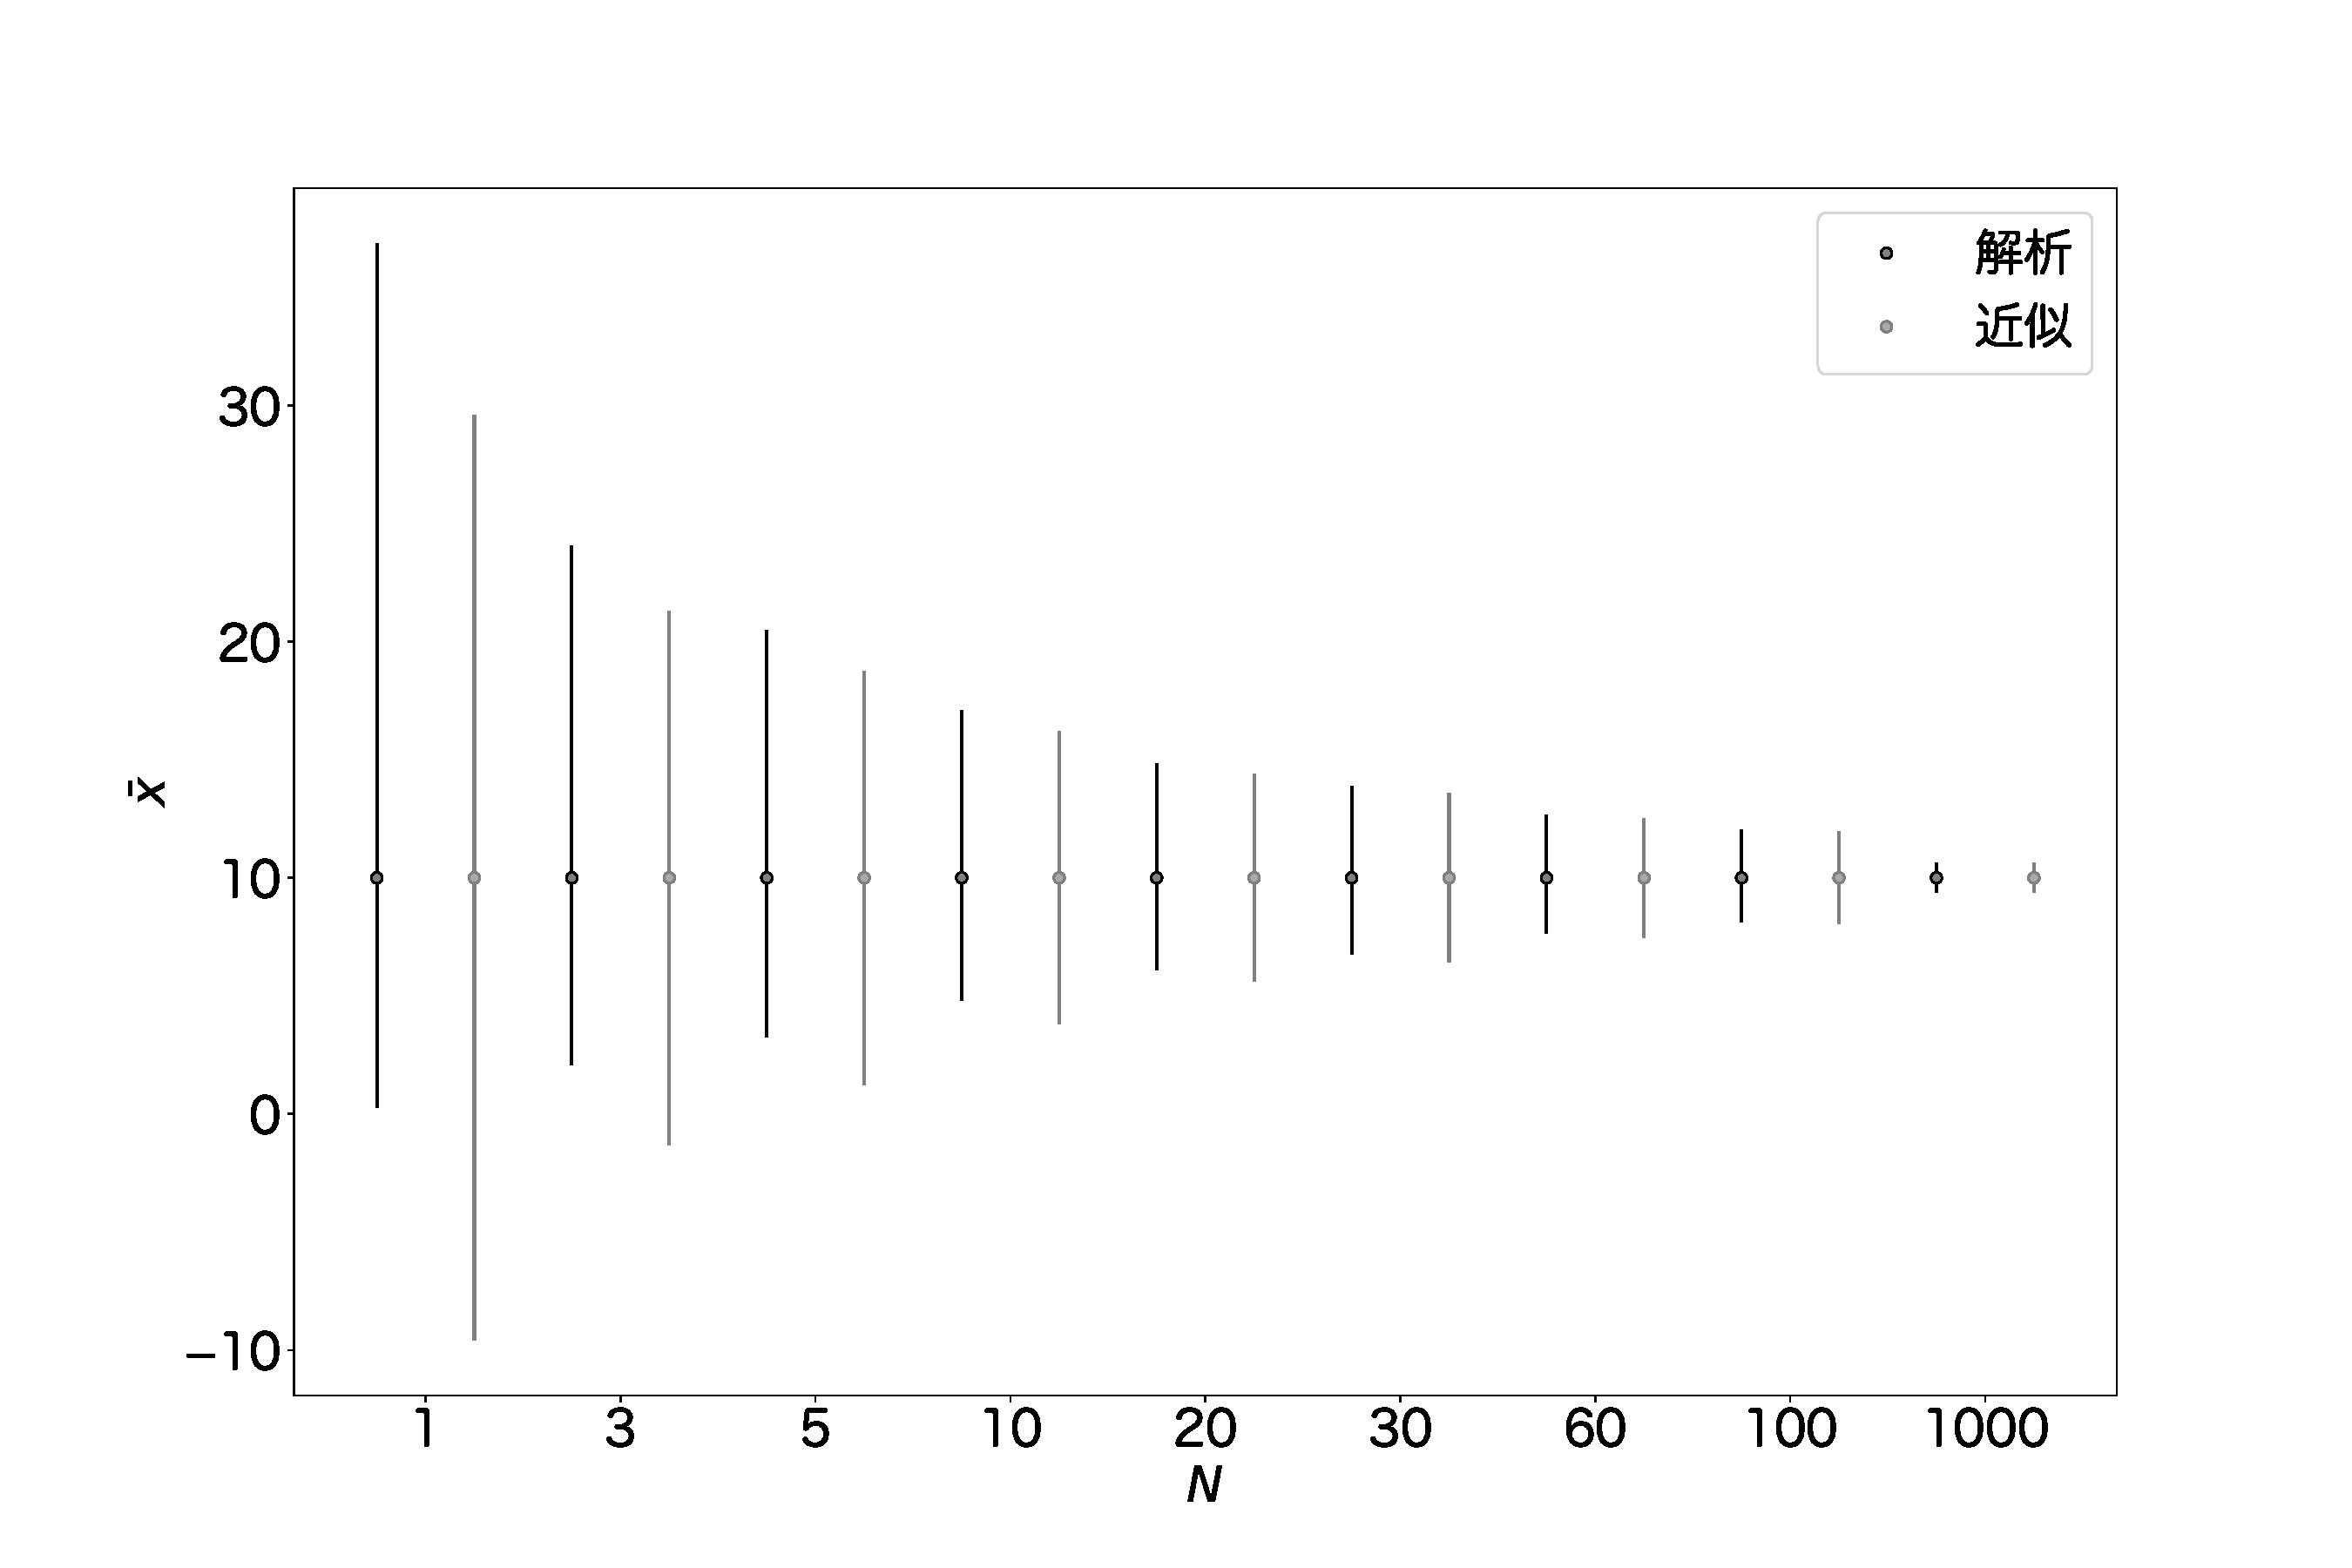
\includegraphics[width=15cm]{./image/12_/confidence_expon_interval.pdf}
        \label{fig:model_predict_CI_interval}
        \caption{解析的な信頼区間と近似によって求められた信頼区間。$1/\lambda=10$とする。横軸にサンプルサイズ。縦軸に、平均値。エラーバーは信頼区間(CI)。}
      \end{center}
    \end{figure}

\section{モデルの選択}
データの分布とモデルの分布が一致しているとき、そのモデルの予測も当たりやすい。
例えば、データがある値の周りに対象に分布していないにもかかわらず、正規モデルを使うと、その予想は当たりにくい。
このことから、データに適したモデルを選ぶ必要があると考えられる。

%ここで、現状のデータからモデルを選択したとして、その予測が当たるかはわからない。
%サンプルサイズが小さいとき、予測が当たりそうなモデルを選ぶことが難しい。
事前実験やこれまでの研究結果から推測し、モデルの分布と標本分布が一致していそうなモデルを選ぶことになる。

モデルを選択できるほどのサンプルサイズを集めて、母集団を予測しやすいモデルを決めることも科学的な成果になりうる。

\subsection{図による比較}
\subsection{AICの比較}

\if 0
\section{標本が統計モデルにより予測可能かを判定する}%統計モデルの性質を使った方法}
%ここまでは、統計モデルの予測がデータと一致することを定量的に評価した。
ここでは、推測に適していないと判断する方法である、統計的仮説検定を紹介する。
この方法は、統計量の一つである統計検定量の統計モデル上での出現しやすさにより、モデルを評価する。
\fi 



\if 0
\section{モデルの種類}

\begin{table}[hbtp]
    \caption{モデル}
    %\label{table:data_type}
    \centering
    \begin{tabular}{ccc}
      \hline
      モデルの仮定  & 棄却域  &  予測区間 \\
      $M(\mu_0,\sigma_0^2)$ $x_1,x_2,\cdots,x_n\sim N(\mu_0,\sigma_0^2)$  \\
      $\mu_0=\bar{x},\sigma_0^2=\frac{1}{n}\sum(x_i-\bar{x})^2$& -  &  - \\
      $\mu_0,\sigma_0$は設定値とする & $\frac{\sqrt{n}|\bar{x}-\mu_0|}{\sigma_0}\sim N(0,1)$  & $\mu_0-z_{\alpha/2}\frac{\sigma}{\sqrt{n}} <\bar{x}<\mu_0+z_{\alpha/2}\frac{\sigma}{\sqrt{n}}$ \\
      $\mu_0$は設定値,$\sigma^2$は未知 & 
      $|\frac{\bar{x}-\mu_0}{\frac{U}{\sqrt{n}}}| > t_{n-1,\frac{\alpha}{2}}$ただし、$U^2=\frac{1}{n-1}\sum(x_i-\bar{x})$
      %$\mu_0=\bar{x},\sigma_0^2=\frac{1}{n}\sum(x_i-\bar{x})^2$ 
      &  \\
      
      \hline
    \end{tabular}
  \end{table}
  \fi